\documentclass[10pt]{article}

\usepackage[applemac]{inputenc}
\usepackage[english]{babel}
\usepackage[T1]{fontenc}
\usepackage{cite, url,color} % Citation numbers being automatically sorted and properly "compressed/ranged".
%\usepackage{pgfplots}
\usepackage{graphics,amsfonts}
\usepackage[pdftex]{graphicx}
\usepackage[cmex10]{amsmath}
% Also, note that the amsmath package sets \interdisplaylinepenalty to 10000
% thus preventing page breaks from occurring within multiline equations. Use:
 \interdisplaylinepenalty=2500
% after loading amsmath to restore such page breaks as IEEEtran.cls normally does.

%% Useful packages for creation of two-column and more complex figures
% Compact lists
\usepackage{enumitem}
\usepackage{booktabs}
\usepackage{fancyvrb}

\usepackage{listings} % inserisce listati di programmi
\definecolor{commenti}{rgb}{0.13,0.55,0.13}
\definecolor{stringhe}{rgb}{0.63,0.125,0.94}
\lstloadlanguages{Matlab}
\lstset{% general command to set parameter(s)
framexleftmargin=0mm,
frame=single,
keywordstyle = \color{blue},% blue keywords
identifierstyle =, % nothing happens
commentstyle = \color{commenti}, % comments
stringstyle = \ttfamily \color{stringhe}, % typewriter type for strings
showstringspaces = false, % no special string spaces
emph = {for, if, then, else, end},
emphstyle = \color{blue},
firstnumber = 1, % numero della prima linea
numbers =right, %  show number_line
numberstyle = \tiny, % style of number_line
stepnumber = 5, % one number_line after stepnumber
numbersep = 5pt,
language = {Matlab}, % per riconoscere la sintassi matlab
extendedchars = true, % per abilitare caratteri particolari
breaklines = true, % per mandare a capo le righe troppo lunghe
breakautoindent = true, % indenta le righe spezzate
breakindent = 30pt, % indenta le righe di 30pt
basicstyle=\footnotesize\ttfamily
}

%Pseudocode package
\usepackage{algorithm}
\usepackage[noend]{algpseudocode}

\usepackage{array}
% http://www.ctan.org/tex-archive/macros/latex/required/tools/
\usepackage{mdwmath}
\usepackage{mdwtab}
%mdwtab.sty	-- A complete ground-up rewrite of LaTeX's `tabular' and  `array' environments.  Has lots of advantages over
%		   the standard version, and over the version in `array.sty'.
% *** SUBFIGURE PACKAGES ***
\usepackage[tight,footnotesize]{subfigure}

\usepackage[top=2cm, bottom=2cm, right=1.6cm,left=1.6cm]{geometry}
\usepackage{indentfirst}

%\usepackage{times}
%\usepackage[active]{srcltx}

\setlength\parindent{0pt}
\linespread{1}

\def\C#1{\mathcal{#1}}

\usepackage{mathtools}
\DeclarePairedDelimiter{\ceil}{\lceil}{\rceil}
\DeclarePairedDelimiter{\floor}{\lfloor}{\rfloor}
\DeclareMathOperator*{\argmin}{arg\,min}
\DeclareMathOperator*{\argmax}{arg\,max}
%\DeclareMathOperator*{\arccos}{arc\,cos}


% Package used to keep inherent figures in the same section
\usepackage{placeins}

\graphicspath{ {images/} }



\begin{document}
\title{Network Analysis and Simulation - Homework 3}
\author{Michele Polese, 1100877}

\maketitle

\section*{Exercise 1 - Queue simulations}
In this exercise the behavior of two different queues is simulated. They are both slotted, the first one has deterministic service, in one slot, and arrivals in each slot distributed in the following way
\begin{equation}
  \mbox{number of arrivals} = 
  \begin{cases}
    2 & \mbox{with probability } a\\
    1 & \mbox{with probability } a\\
    0 & \mbox{with probability } 1-2a
  \end{cases}
  \label{eq:queue1arr}
\end{equation}
Therefore the average rate of arrivals is $\lambda_1 = 3a$, the service rate $\mu_1 = 1$ and $\rho = \frac{\lambda_1}{\mu_1} = 3a$. 
The goal of the simulation is to study as first the throughput-delay tradeoff, in particular for $a \in [0, 1/3]$ the delay of the queue is studied as a function of $\rho$. Note that for $a = 1/3$ then $\rho = 1$, therefore the queue is unstable and the result of the simulation would not be meaningful. Thus the extreme points of the interval $[0, 1/3]$ are not studied. 

The queue behaves as follows. At the beginning of each slot, if there's at least one user, the first user who arrived is served. Then the arrivals take place, with the probabilities of~\eqref{eq:queue1arr}, and finally the number of users in the queue is sampled. Since the service process is deterministic of $N_s$ solts, there's a counter that in presence of users in the queue increases at each slot of one unit until it reaches the given $N_s$. In particular the users cannot be served in the same slot in which they arrive. The slot in which they begin their service time already counts as 1, therefore the counter of the remaining slots is initialized to 1 and not to 0. Since in this queue the service time $N_s = 1$, then the first slot in which a user enters in service is also the slot in which it leaves the queue. However the MATLAB function that simulates the queue is general and it can handle any deterministic service time. 

In this implementation the delay of each departed packet is measured with the help of a FIFO queue as data structure. In MATLAB this is an array whose last position is filled with the couple $(slot, n)$ at each arrival, where $slot$ is the index of the time slot in which there is the $n$-th arrival. If there are two arrival, then they are both inserted in the queue with the same $slot$ value and an increasing $n$. When a there's a departure, instead, the first position of the queue is read, and the difference between current slot index and the $slot$ value is stored in an array. Then the first couple of the queue is popped out and every element shifts by one. 

The function that simulates the queue finally returns an array with the number of users for each slot and a second one with the delay for each departed user, in order to let the main class handle statistics. In particular, for each value of $a$ (which is sampled in $[0.1, 0.9]/3$), I repeat 100 indipendent simulations, each of length $n_{slot} = 10^6$ slots. For each simulation, given the number $n_{d}$ of departed users, I compute the mean delay as 
\begin{equation}
  dl_{sim} = \frac{1}{n_d} \sum_{i = 0}^{n_d} dl_{user_i}
\end{equation}
and then I average over the 100 simulations to get a lower variance. The results are in Figure~\ref{fig:queue_a}.
I also studied the behavior of one realization of the queue in $10^4$ slots, whose occupancy is in Figure~\ref{fig:queue_a_real}.

\begin{figure}[h!]
\centering
  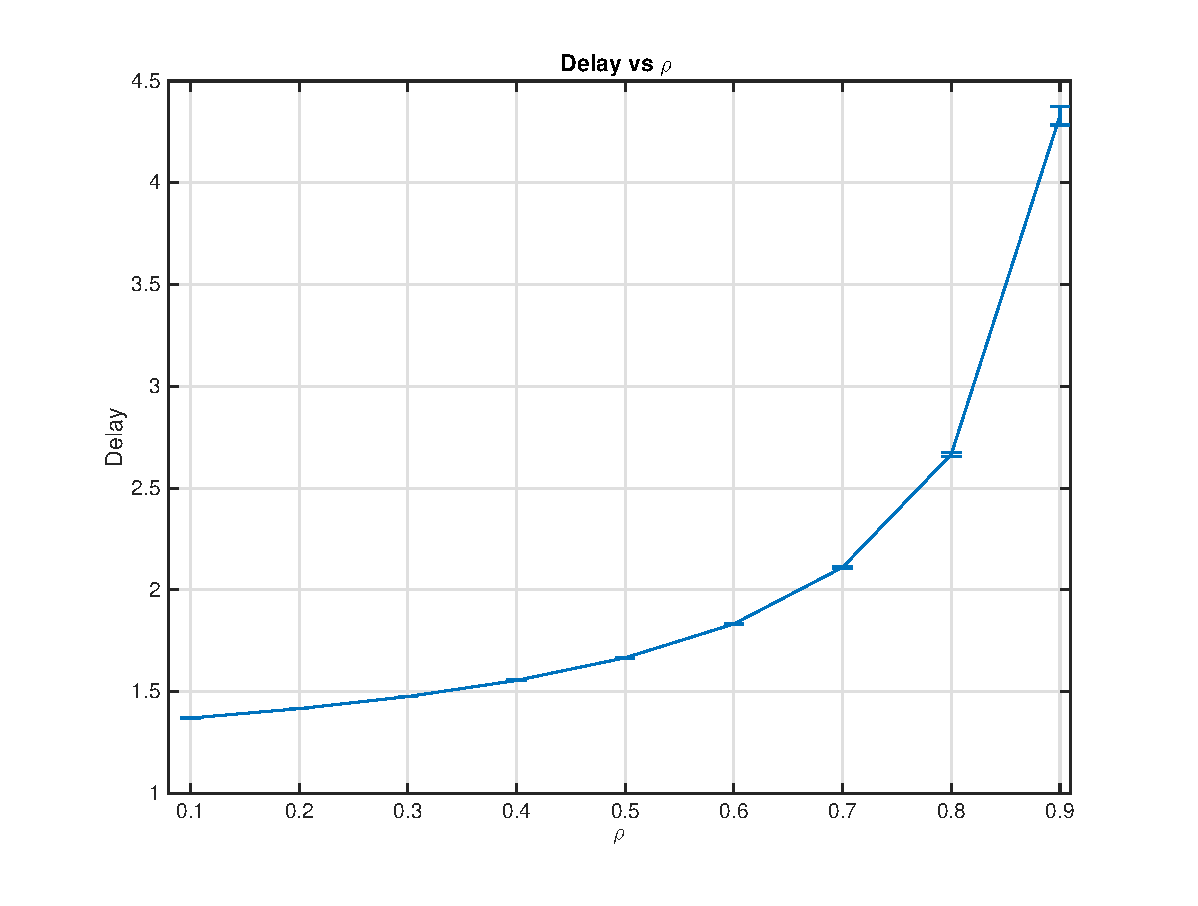
\includegraphics[width = 0.6\textwidth]{queue_a_dl}
  \caption{Delay vs. utilization factor $\rho$}
  \label{fig:queue_a}
\end{figure}

\begin{figure}[h!]
\centering
  \subfigure[Realization of the queue for $a = 0.25, \rho = 3/4$]{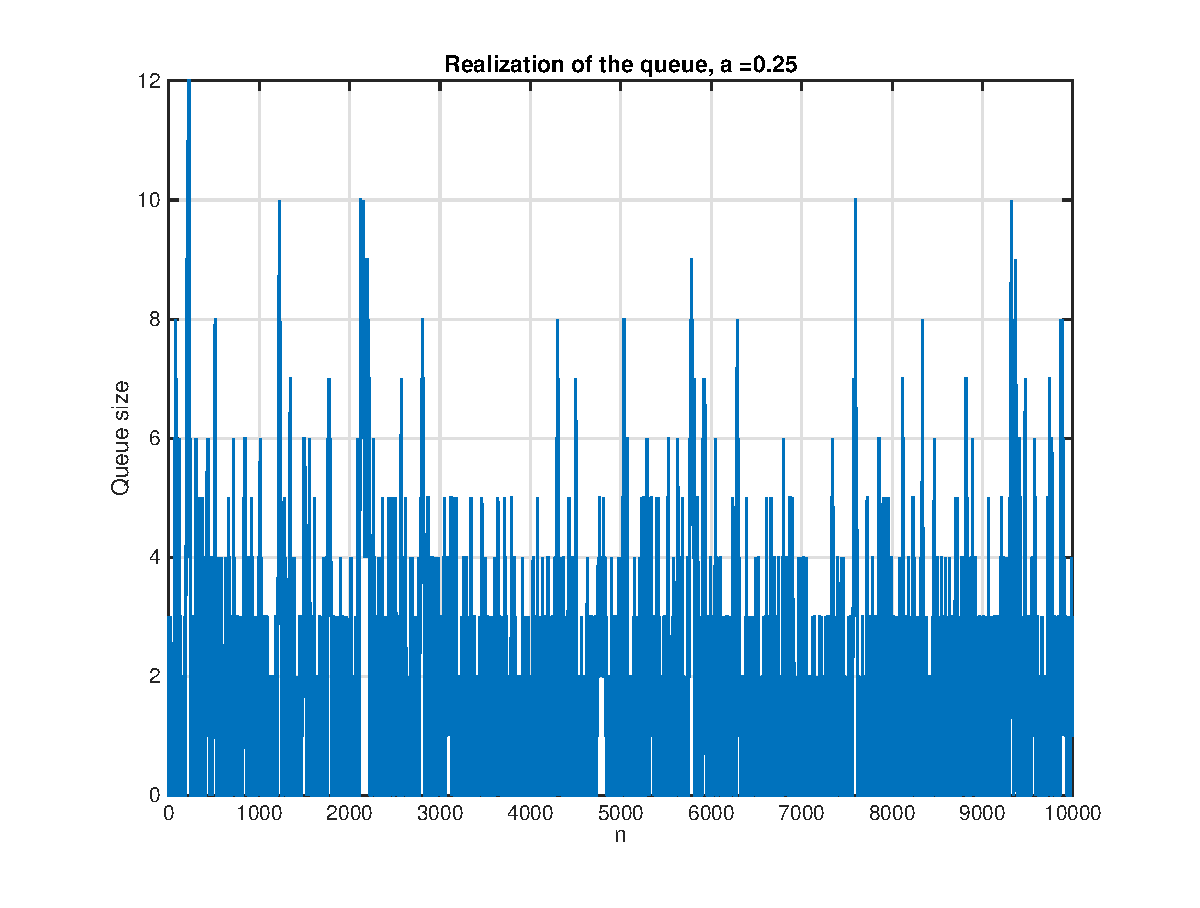
\includegraphics[width = 0.45\textwidth]{queue_a25}}
  \subfigure[Realization of the queue for $a = 1/3, \rho = 1$]{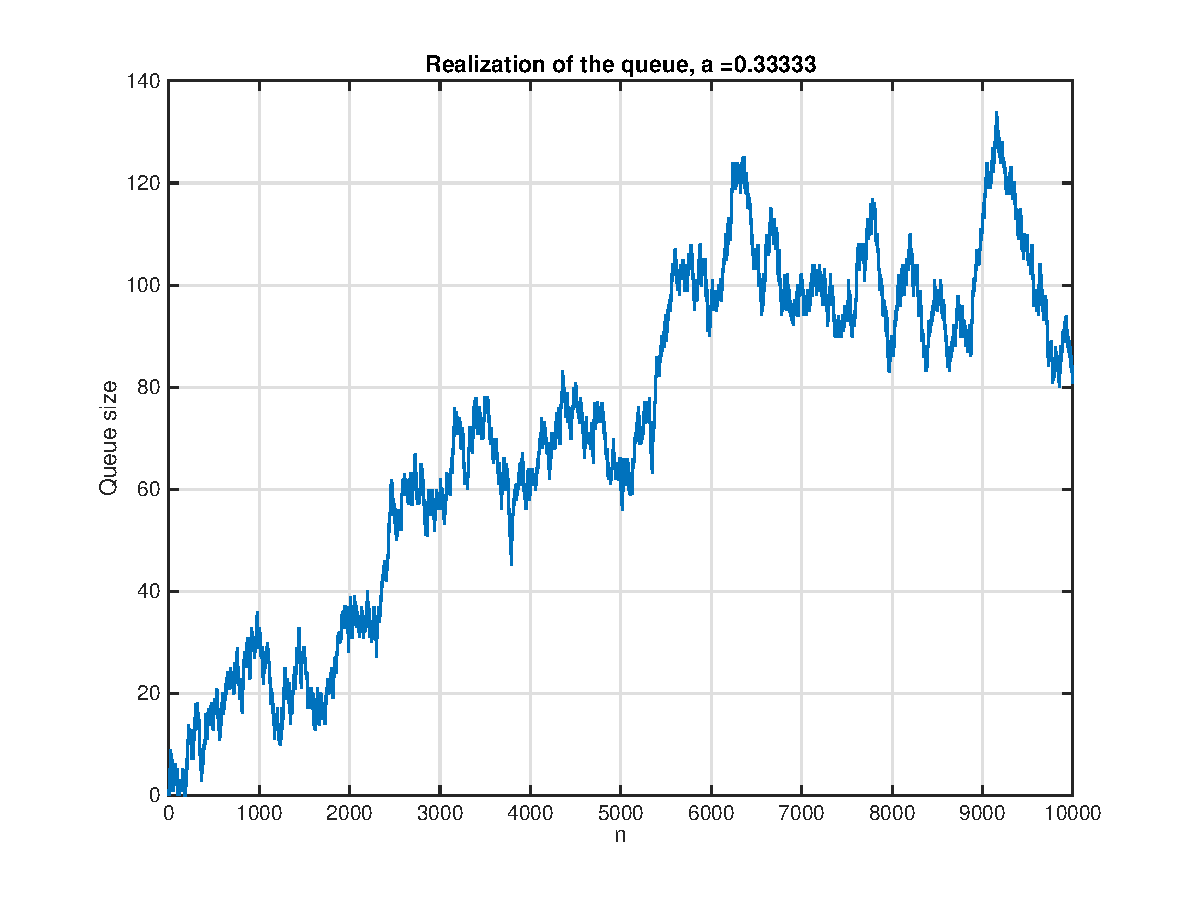
\includegraphics[width = 0.45\textwidth]{queue_a33}}
  \subfigure[Realization of the queue for $a = 0.5, \rho = 1.5$]{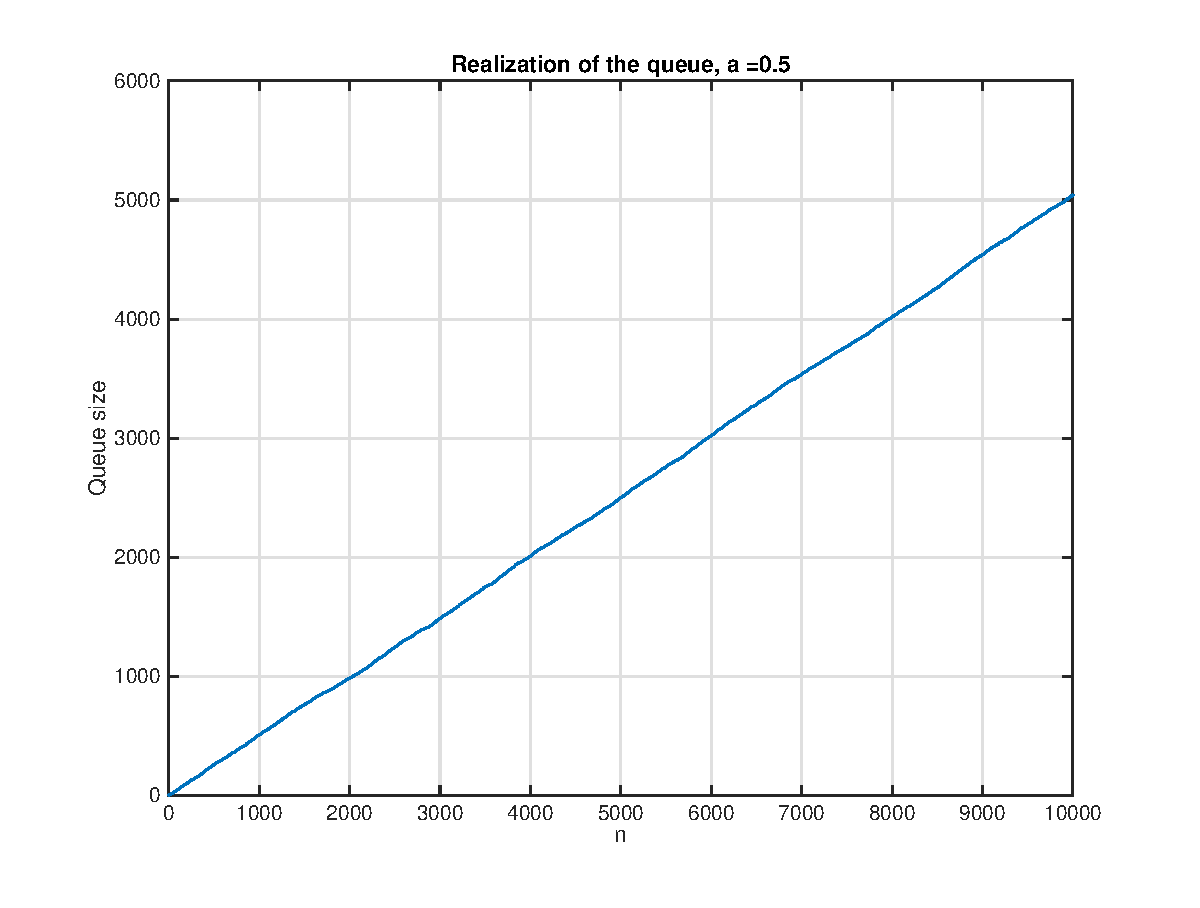
\includegraphics[width = 0.45\textwidth]{queue_a50}}
  \caption{Realization of the queue for $10^4$ slots}
  \label{fig:queue_a_real}
\end{figure}


The second queue, instead, has a bernoulli arrival process, with one arrival with probability $1/2$ in each slot, and a geometric service time of average $1/b$. Since the arrival rate is $\lambda_2 = 1/2$ and the service rate is $\mu_2 = b$, then the utilization factor is $\rho = \frac{1}{2b}$. Also for this queue I studied the throughput-delay trade-off, with the events happening in each slot as in the previous queue and with delay measured for each departed packet with a FIFO queue. Note that since departures are geometric, they are memoryless and the counter of the number of slots spent in service is useless. Therefore at every slot, if there's at least one user, it departs with probability $b$ and it remains in service with probability $1-b$. 

The results are in Figure~\ref{fig:queue_b}, while the realizations of the queue in $10^4$ slots are Figure~\ref{fig:queue_b_real}.

\begin{figure}[h!]
\centering

  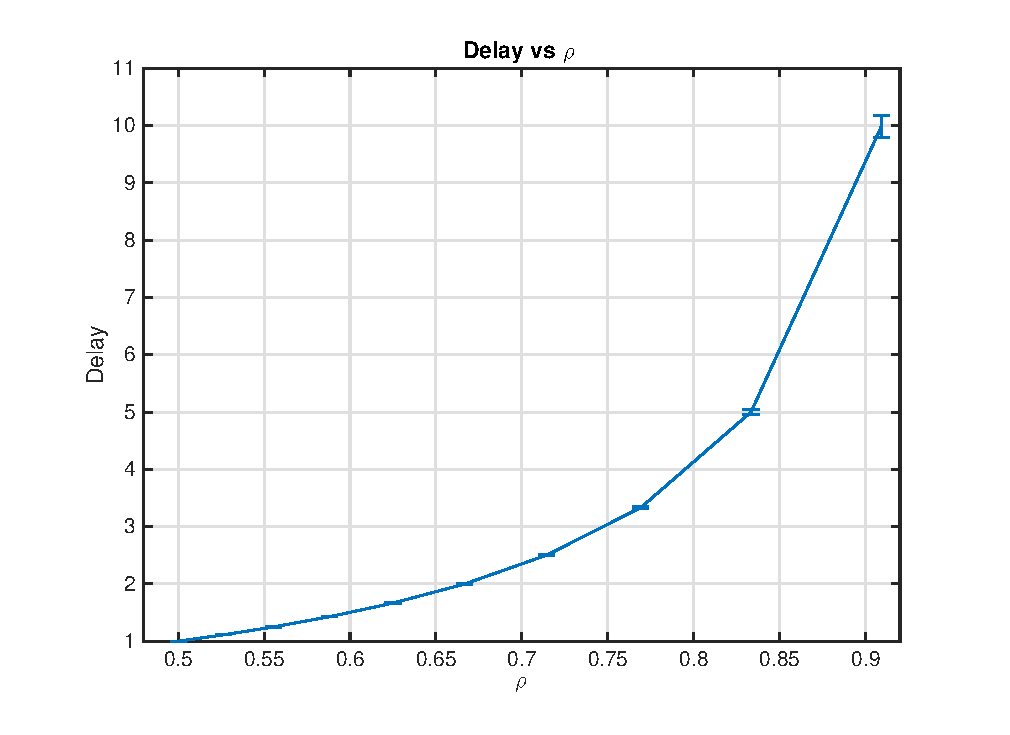
\includegraphics[width = 0.6\textwidth]{queue_b_dl}
  \caption{Delay vs. utilization factor $\rho$}
  \label{fig:queue_b}
\end{figure}

\begin{figure}[h!]
\centering
  \subfigure[Realization of the queue for $b = 3/4, \rho = 2/3$]{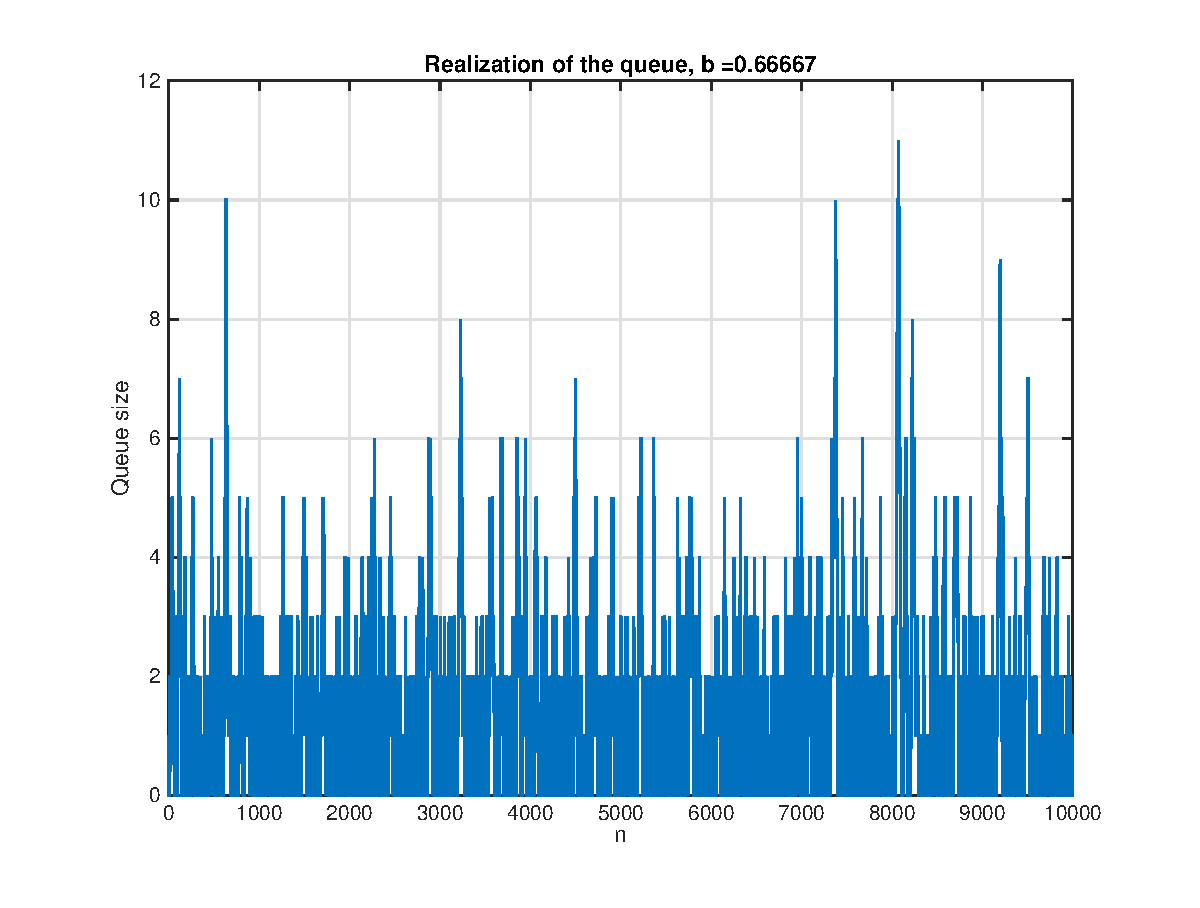
\includegraphics[width = 0.45\textwidth]{queue_b66}}
  \subfigure[Realization of the queue for $b = 1/2, \rho = 1$]{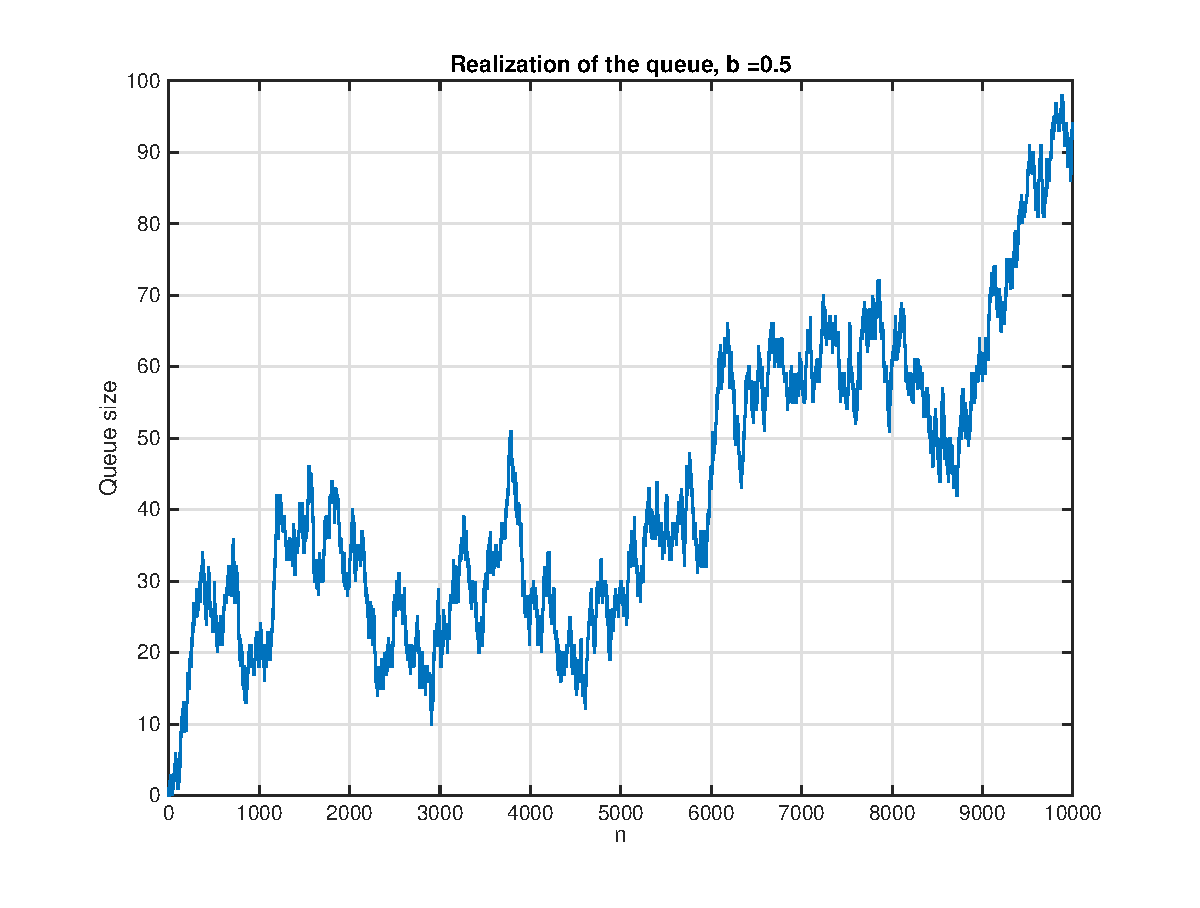
\includegraphics[width = 0.45\textwidth]{queue_b50}}
  \subfigure[Realization of the queue for $b = 1/3, \rho = 1.5$]{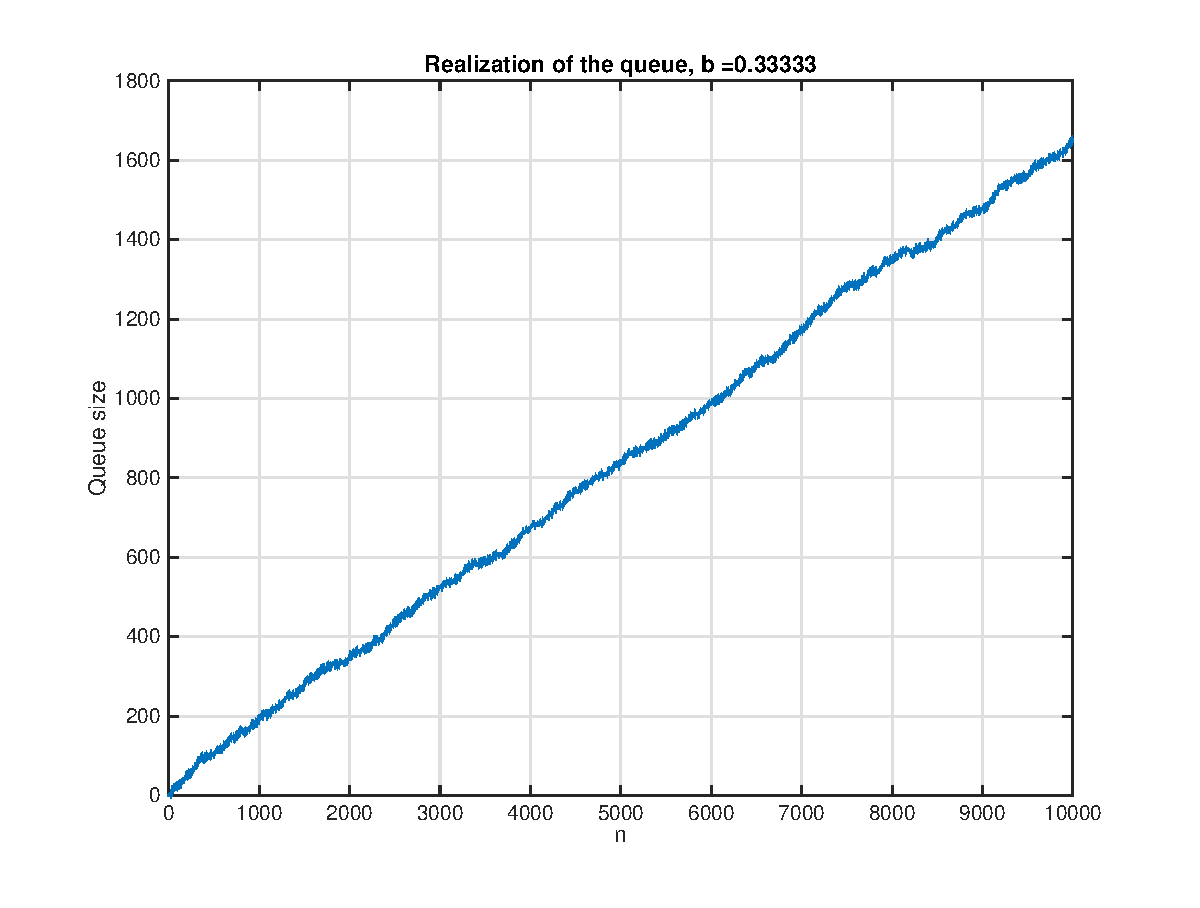
\includegraphics[width = 0.45\textwidth]{queue_b33}}
  \caption{Realization of the queue for $10^4$ slots}
  \label{fig:queue_b_real}
\end{figure}


The second element that is studied on each of these queues is the probability of overflow with a fixed sized queue, for stable $\rho$. The probability of overflow is given by 
\begin{equation}
  P_{of} = \frac{\mbox{dropped packets}}{\mbox{dropped packets} + \mbox{served packets}}
\end{equation}
where the denominator is equal to the total number of arrivals in the system. 

I studied this probability with 2 dedicated functions for each type of queue, which handle the departures and arrivals as before but don't track the number of users in the system for each slot and the delay metric in order to speed up the simulation. The length of each simulation is indeed a critical issue. In order to estimate a very low probability very long simulations must be run, because otherwise the number of observed events would be to small to provide a reliable estimate. In particular, for each simulation with $n_{arr}$ arrivals, a general result from \cite{leb} states that if the number of drop events observed is $z \ge 6$ and $n_{arr} - z \ge 6$ and if the events are iid then it is possible to apply a normal approximation for the confidence interval at a certain level $\gamma$, i.e.
\begin{equation}
  \begin{cases}
  L(z) \approx \frac{z}{n} - \frac{\eta}{n}\sqrt{z\left(1 - \frac{z}{n}\right)} \\
  U(z) \approx \frac{z}{n} + \frac{\eta}{n}\sqrt{z\left(1 - \frac{z}{n}\right)}
  \end{cases}
\end{equation}
with $\eta$ such that $N_{0,1}(\eta) = \frac{1+\gamma}{2}$.

However the events involved in the queue overflow are not independent, since when there is a dropping event it is probable that the following arrival will be dropped too. Therefore in order to compute a confidence interval on the $P_{of}$ I repeated $N$ times for each supposed length the simulation of a queue with $n_{slots} = \frac{100}{\lambda_i \hat{P}_{of}}$, where $\hat{P}_{of}$ is the target probability of overflow of $10^{-5}$, in order to observe on average at least $\frac{100}{\lambda_i}$ events. 

The experiment is repeated $N = 160$ times, in order to reduce the variance, and the final probability of overflow for a given size is computed as the sample mean of the $N$ probability of overflow. The size chosen is the one that guarantees that the upper bound of the confidence interval for the sample mean estimator is below the required threshold of $10^{-5}$. 

In Figure~\ref{fig:pofA} it can be seen that for the first queue, $a = 0.25$, the required size is 14, while Figure~\ref{fig:pofB} shows that for the geometric queue, $b = 0.75$, the size that guarantees $P_{of} < 10^{-5}$ is 13.

\begin{figure}[h!]
\centering
  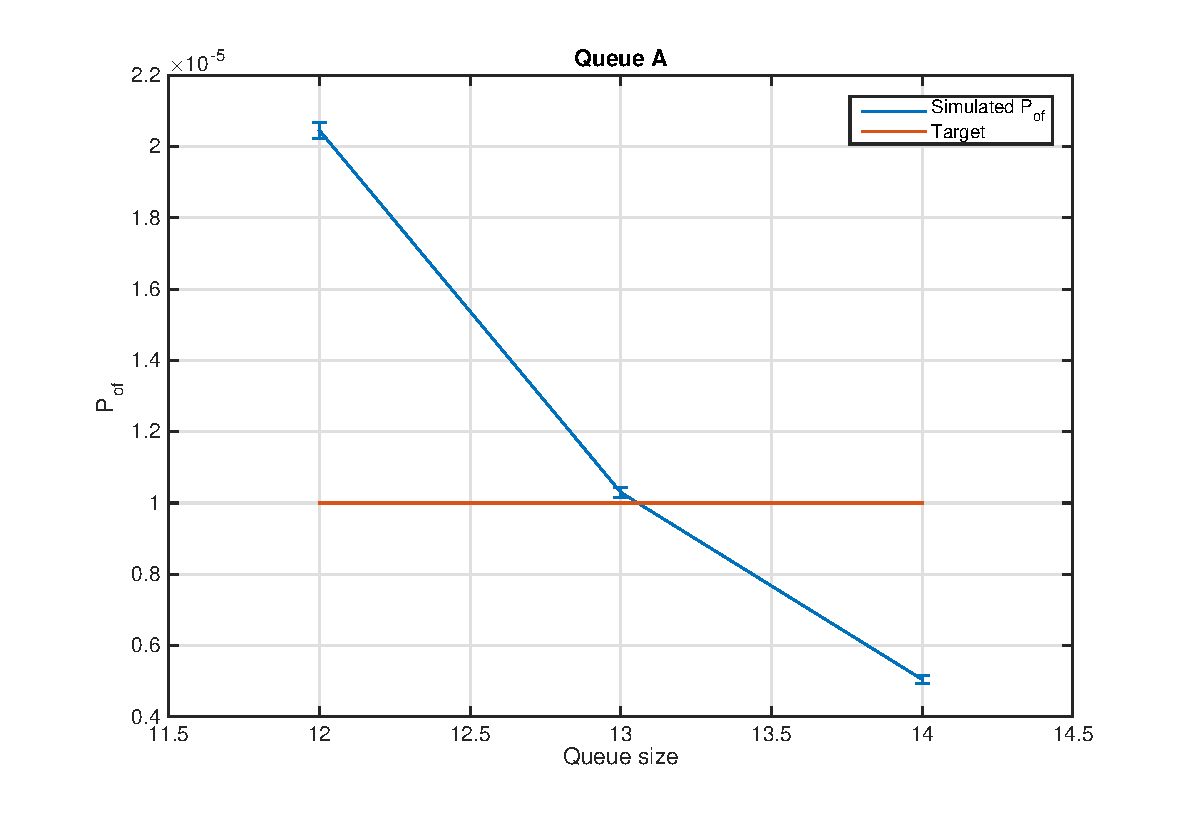
\includegraphics[width = 0.7\textwidth]{queue_a_of}
  \caption{$P_{of}$ of the queue A for $a = 0.25, \rho = 0.75$}
  \label{fig:pofA}
\end{figure}

\begin{figure}[h!]
\centering
  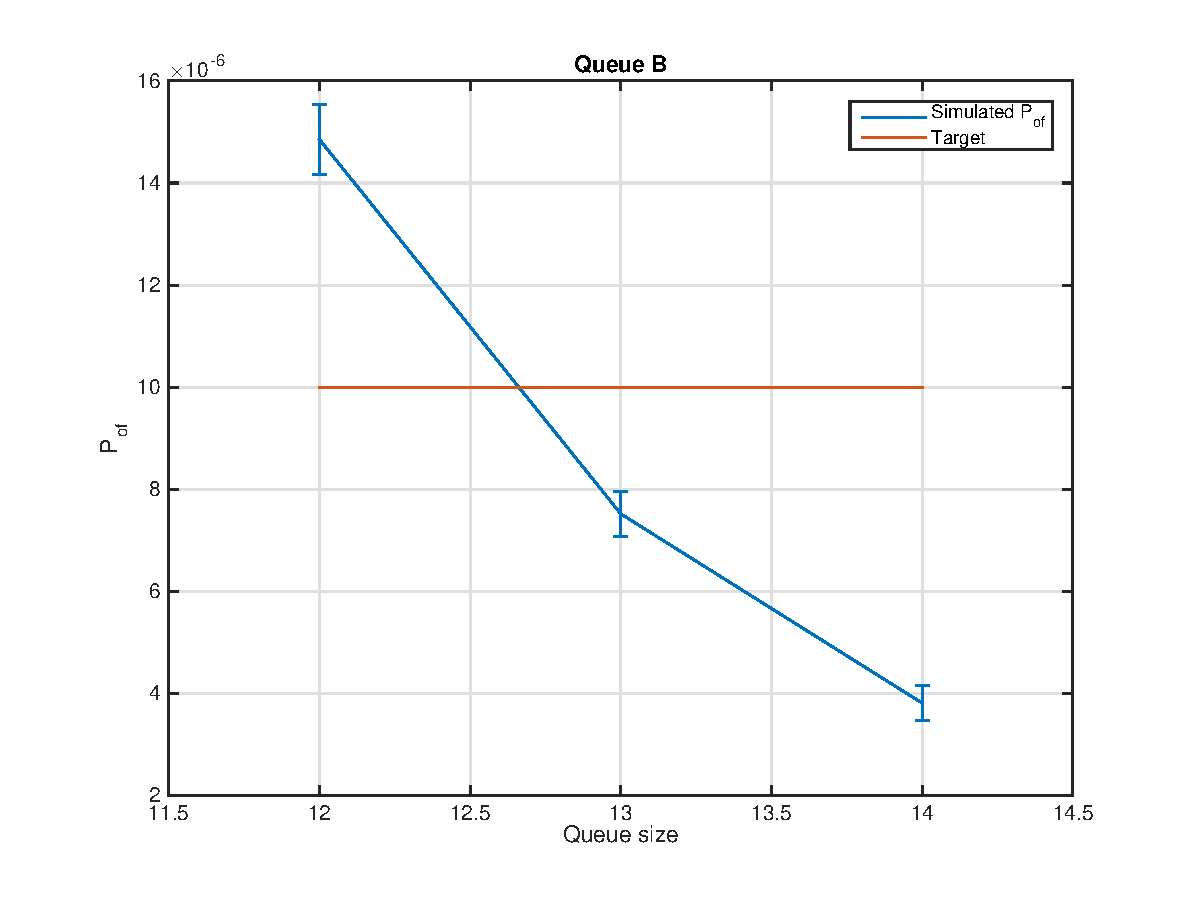
\includegraphics[width = 0.7\textwidth]{queue_b_of}
  \caption{$P_{of}$ of the queue A for $b = 0.75, \rho = 2/3$}
  \label{fig:pofB}
\end{figure}

\clearpage

\section*{Cellular system and Aloha}
In a slotted Aloha system it is interesting to study which is the probability that some transmission are successful even in presence of interferers. 
Each user in the system which has to communicate with a central base station is characterized by the following quantities:
\begin{itemize}
\item distance $r$ from the BS. Since the users are uniform in a circle of radius 1, then the probability density function of this distribution is $h(r) = 2r$.
\item $\eta$ power loss law exponent, which in the following simulations is set to 4
\item a log-normal random variable $e^{\xi}$ that describes shadowing, with $\xi \sim N_{0,\sigma^2}$. Note that the given $\sigma_{dB}= 8$ is in dB, thus $\sigma = (0.1 \log_e(10))\sigma_{dB}$
\item a Rayleigh distributed r.v. with unit power $\sigma_R = 1$. Note that a Rayleigh r.v. can be generated as $\sigma_R \sqrt{-2*\log_e(X)}$ with $X \sim N_{0,1}$.
\end{itemize}
The received power from a transmitter at distance $r$ is then $P_R = R^2 e^{\xi} K r^{-\eta} P_T$. The constant term $K P_T$ and the exponent $\eta$ are equal for all the users, and also the Rayleigh fading and the log-normal shadowing are iid. 

Then the signal to interference ratio of a user against $k$ interferers can be expressed as
\begin{equation}
  SIR = \frac{P_{R0}}{\sum_{i=1}^{k} P_{Ri}} = \frac{R_0^2 e^{\xi_0}}{\sum_{i = 1}^{k}R_i^2 e^{\xi_i}\left(\frac{r_0}{r}\right)^{\eta}}
\end{equation}
There is a successful transmission for this user with probability 
\begin{equation}
  P_s = P[SIR > b]
  \label{eq:ps}
\end{equation}
with $b$ a suitable threshold, that in the following simulations will be set to 6 and 10 dB. 

This quantity can be computed analytically as it is done in \cite{capture} and the final result of the probability of having a success for a user at distance $r_0$ given that $n$ packets are transmitted (thus $n-1$ interferers) is
\begin{equation}
  P_n(r_0) = \int_{-\infty}^{\infty} \frac{d\xi_0}{\sqrt{2\pi}\sigma} e^{-\frac{\xi_0^2}{2\sigma^2}}[I(\xi_0, r_0)]^{n-1}
\end{equation}
with 
\begin{equation}
  I(\xi_0, r_0) = \int_{-\infty}^{\infty} \frac{d\xi}{\sqrt{2\pi}\sigma}e^{-\frac{\xi^2}{2\sigma^2}} \int_{0}^{1} \frac{h(r) dr}{1+be^{\xi - \xi_0}\left(\frac{r}{r_0}\right)^{-\eta}}
  \label{eq:I}
\end{equation}
Then the capture probability, that describes the probability that the strongest transmission can be successfully received even with $n-1$ interferers, is
\begin{equation}
  C_n = \int_0^1 nP_n(r_0)h(r_0) dr_0 = \int_{-\infty}^{\infty} \frac{d\xi_0}{\sqrt{2\pi}\sigma} e^{-\frac{\xi_0^2}{2\sigma^2}} \int_0^1 n h(r_0) [I(\xi_0, r_0)]^{n-1} dr_0
  \label{eq:cn}
\end{equation}

In this homework these probabilities are evaluated using a Montecarlo simulation exaclty computed with numerical integration, for a total number of users $n$ up to 30. The Montecarlo simulation computes directly the SIR and compares it to the desired threshold. In particular, in order to speed up the simulation, at each iteration the simulator generates the complete set of random variables as described previously for all the $N_{tot} = 30$ users. Then it computes the SIR as if there were 2 users, 3 users and so on, sampling from the $N_{tot}$ random variables, and compares it with the threshold $b$. It uses a matrix $\mathbf{P}$ of size $n_{sim} \times N_{tot}$ in order to store at each iteration of the simulation $i$ the value
\begin{equation}
P(i, n) = 
\begin{cases}
  n & \mbox{if } SIR > b \mbox{ with } n \mbox{ packets transmitted}\\
  0 & \mbox{otherwise}
\end{cases}
 \quad n = 2, \dots, N_{tot}
\end{equation}
while $P(i, 1) = 1$ since if there is only one transmission it is successful (in this analysis the noise is not taken into account).
Then each for each column $n$ of the matrix the estimate of $C_n$ is computed as
\begin{equation}
  \hat{C}_n = \frac{1}{n_{sim}} \sum_{i = 0}^{n_{sim} - 1} P(i, n)
\end{equation}
and results are in Figure~\ref{fig:aloha_monte}.

\begin{figure}[h!]
  \centering
  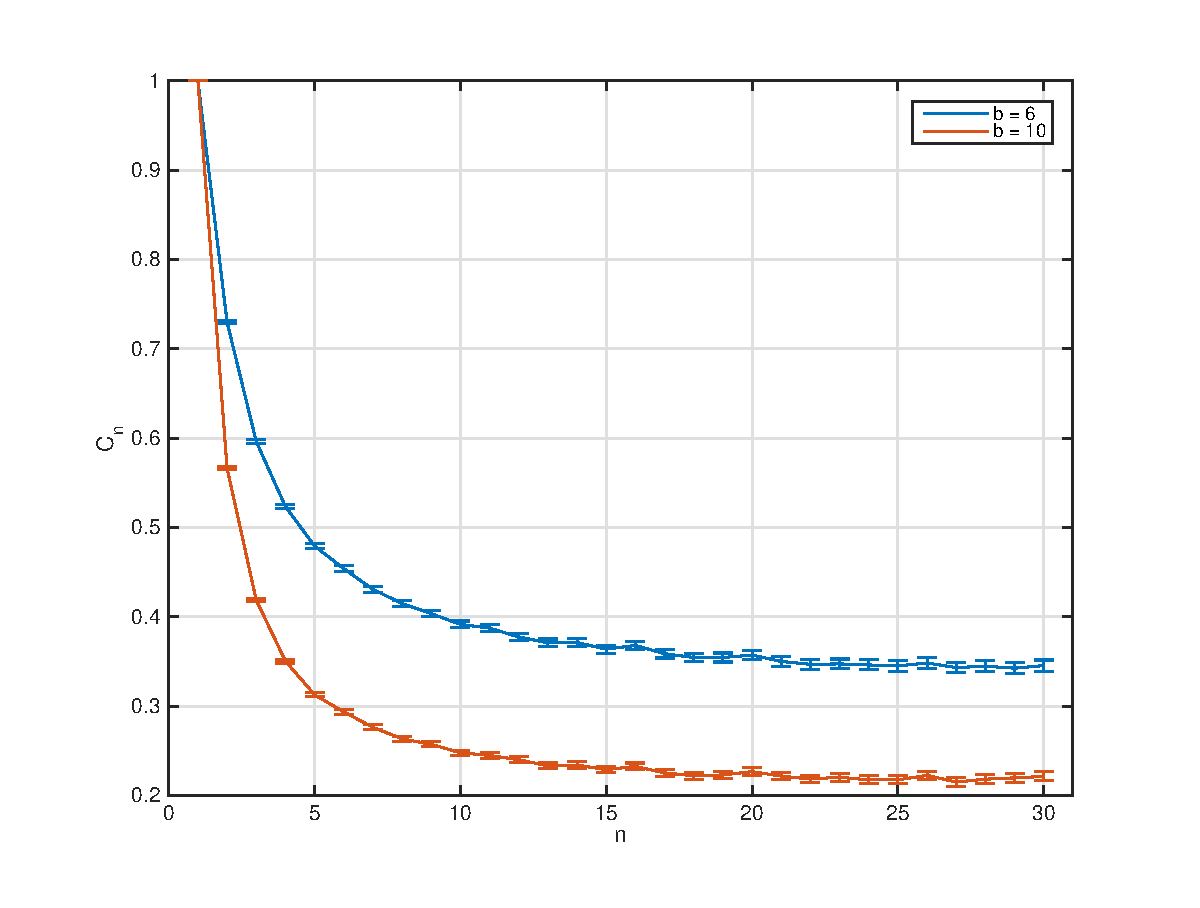
\includegraphics[width = 0.6\textwidth]{aloha_monte}
  \caption{Montecarlo simulation results for capture probability in Slotted Aloha, $b = 6, 10$ dB}
  \label{fig:aloha_monte}
\end{figure}

The throughput of the system is computed by averaging the $C_n$ of each simulation with a Poisson distribution of mean $G$, the offered traffic, i.e.
\begin{equation}
  S = \sum_{i = 0}^{30} \frac{G^{i} e^{-G}}{i!} C_i 
  \label{eq:aloha_S}
\end{equation}
and computing the sample mean of the throughput at each iteration. The results are in Figure~\ref{fig:aloha_monte_S}.

\begin{figure}[h!]
  \centering
  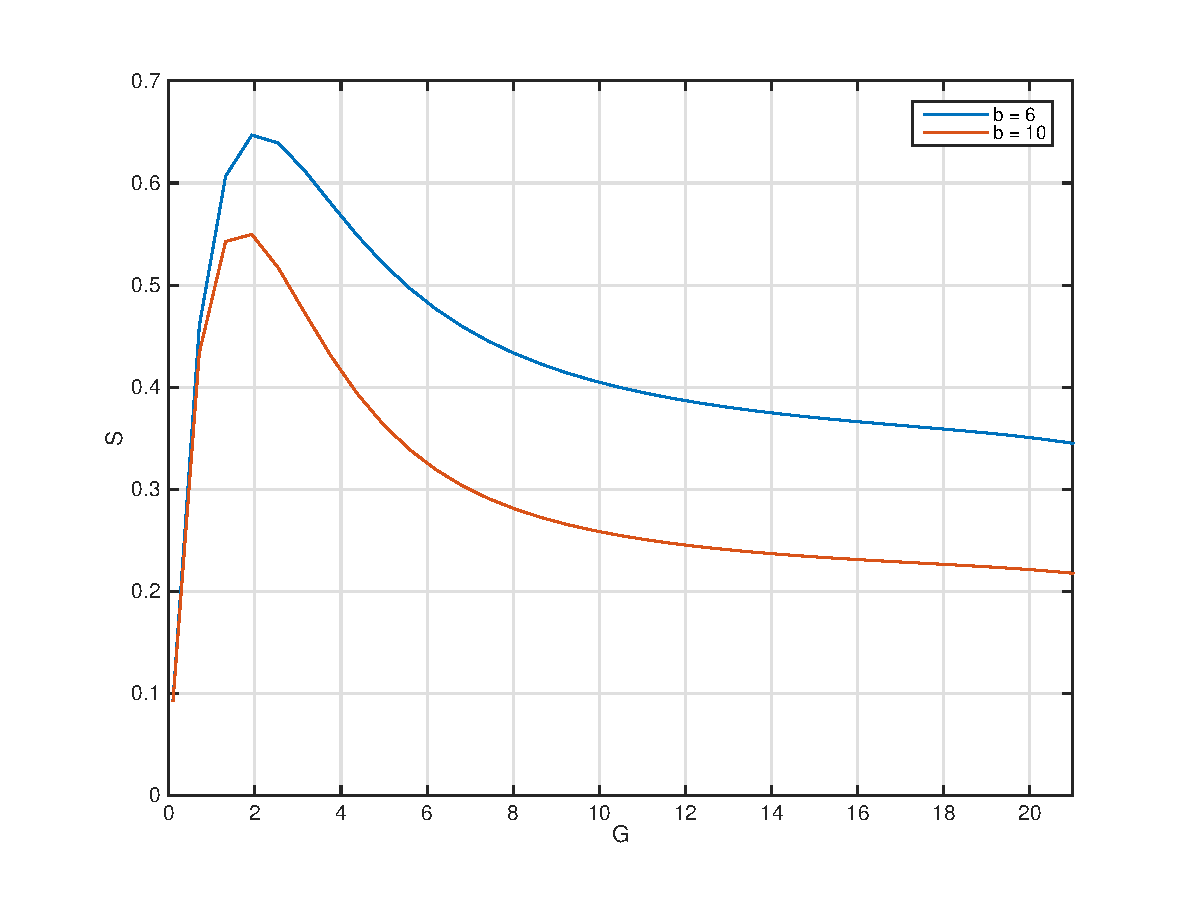
\includegraphics[width = 0.6\textwidth]{aloha_monte_S}
  \caption{Montecarlo simulation results for throughput in Slotted Aloha, $b = 6, 10$ dB}
  \label{fig:aloha_monte_S}
\end{figure}

I also computed the results of Equation~\eqref{eq:cn} with numerical integration, using Gauss-Legendre and Gauss-Hermite quadrature formulas. The derivation is as follows. Let $h(r) = h(r_0) = 2r$ because of the uniform distribution of the users in a circular cell of radius 1. Then
\begin{eqnarray}
  C_n = \int_{-\infty}^{\infty} \frac{d\xi_0}{\sqrt{2\pi}\sigma} e^{-\frac{\xi_0^2}{2\sigma^2}} \int_0^1 n 2 r_0 dr_0 \left[
  \int_{-\infty}^{\infty} 
  \frac{d\xi}{\sqrt{2\pi}\sigma} 
  e^{-\frac{\xi^2}{2\sigma^2}} 
  \int_{0}^{1} 
  \frac{2r dr}{1 + b e^{\xi - \xi_0} \left( \frac{r}{r_0} \right)^{-\eta}}
  \right]^{n-1}
  = \\
  \int_{-\infty}^{\infty} \frac{dx_1}{\sqrt{\pi}}e^{-x_1^2}
  \int_{-1}^{1} n 0.5 (x_2 + 1) dx_2
  \left[
  \int_{-\infty}^{\infty} \frac{dx_3}{\sqrt{\pi}}e^{-x_3^2}
  \int_{-1}{1} \frac{0.5(x_4+1)}{1 + b e^{\sqrt{2}\sigma(x_3 - x_1)}\left( \frac{x_4+1}{x_2+1} \right)^{-\eta}}
  \right]^{n-1}
\end{eqnarray}
with 
\begin{eqnarray*}
x_1 &=& \frac{\xi_0}{\sqrt{2}\sigma}, \, \sqrt{2}\sigma dx_1 =  d\xi_0 \\
x_3 &=& \frac{\xi}{\sqrt{2}\sigma}, \, \sqrt{2}\sigma dx_3 = d\xi \\
x_2 &=& 2(r_0 + 1), \, 0.5 dx_2 = dr_0 \\
x_4 &=& 2(r + 1), \, 0.5 dx_4 = dr
\end{eqnarray*}

The results are in Figure~\ref{fig:aloha_GQR}, while the throughput computed as in~\eqref{eq:aloha_S} is in Figure~\ref{fig:aloha_GQR_S}.

\begin{figure}[h!]
  \centering
  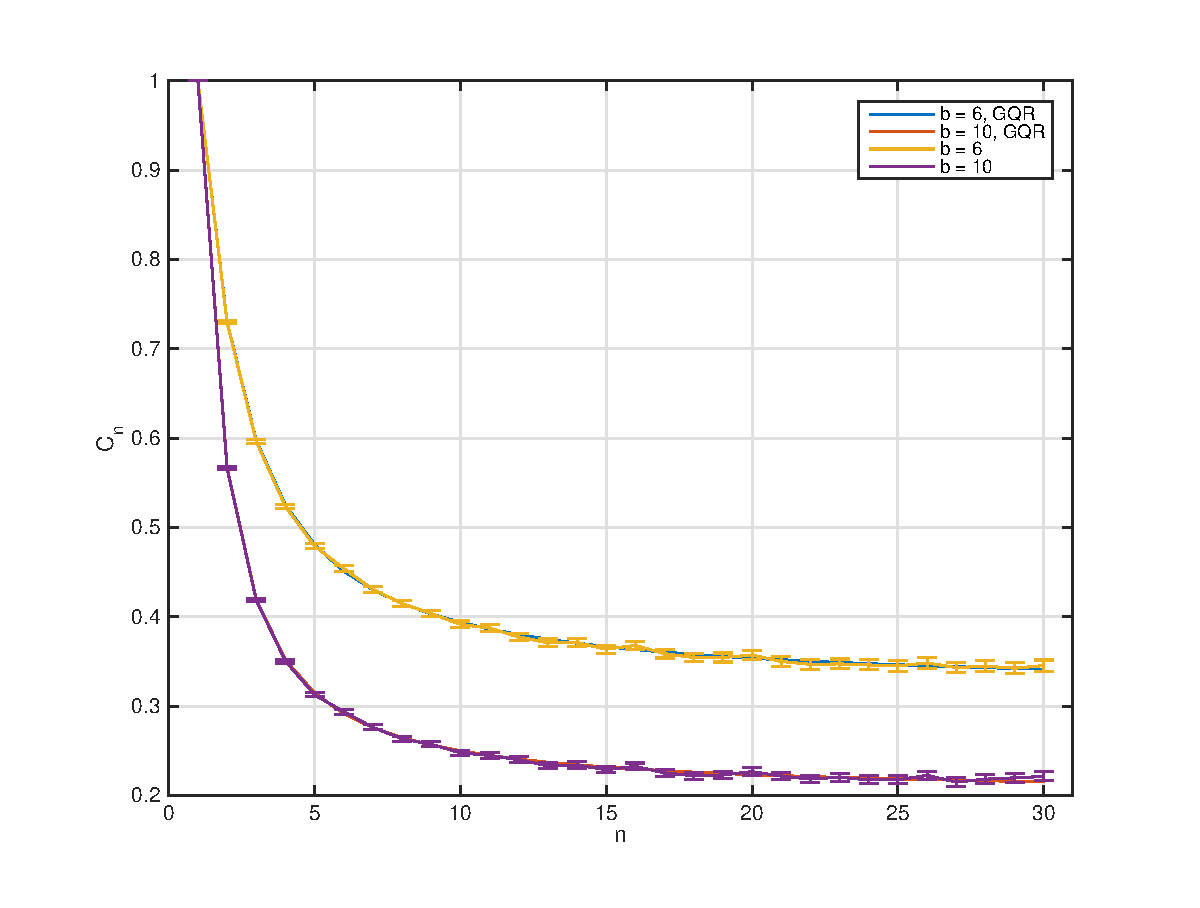
\includegraphics[width = 0.6\textwidth]{aloha_GQR}
  \caption{Montecarlo simulation and numerical integration results for capture probabilities in Slotted Aloha, $b = 6, 10$ dB}
  \label{fig:aloha_GQR}
\end{figure}

\begin{figure}[h!]
  \centering
  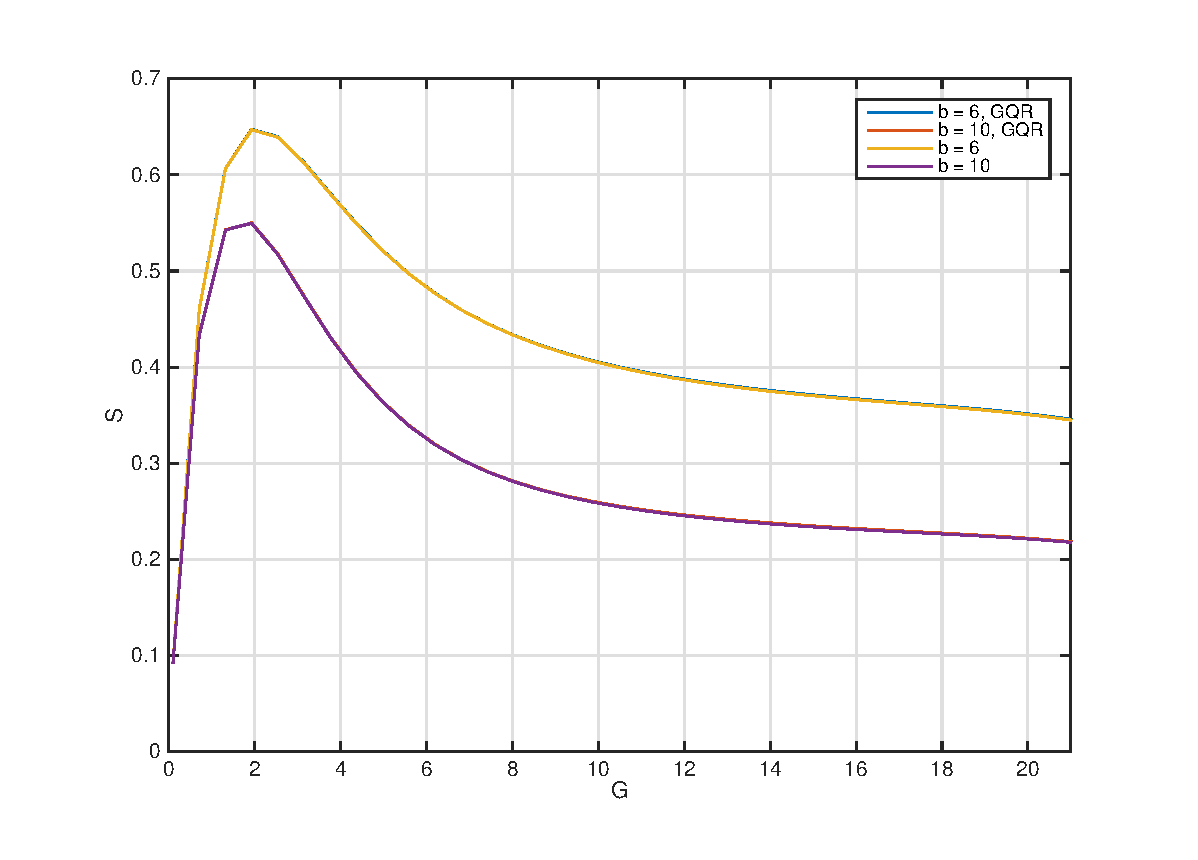
\includegraphics[width = 0.6\textwidth]{aloha_GQR_S}
  \caption{Montecarlo simulation and numerical integration results for throughput in Slotted Aloha, $b = 6, 10$ dB}
  \label{fig:aloha_GQR_S}
\end{figure}

The second study of this exercise regards the simulation of interference in a cellular environment, with interfering users which are present only in the neighborhood cells where the same frequency of the central cell is reused. Four different reuse schemes are used, with $N = \{1, 3, 4, 7\}$ the number of cells with different frequencies in the system.

An assumption is done, which is that the interfering cells are only the 6 closest ones. In particular a user in each cell is active with probability $\alpha$ and inactive with probability $1-\alpha$. Therefore the number of active interferers with a given traffic level $\alpha \in [0,1]$ is a binomial $Bin(6, \alpha)$. The central-cell user experiences an outage when the SIR falls below a threshold, which is set to $b = \{6, 10\}$ dB. It can be computed as $1 - P_{s}$ with $P_{s}$ defined as in Equation~\eqref{eq:ps}. In particular the probability that the user in the central cell transmits successfully, given its position $r_0$, is 
\begin{eqnarray}
  P_s(r_0) = \int_{-\infty}^{\infty} \frac{d\xi_0}{\sqrt{2\pi}\sigma} e^{-\frac{\xi_0^2}{2\sigma^2}} 
  \sum_{i = 0}^{6} \binom{6}{i} (1 - \alpha)^{6-i} \left(\alpha I(r_0, \xi_0) \right)^{i} = \\
  \int_{-\infty}^{\infty} \frac{d\xi_0}{\sqrt{2\pi}\sigma} e^{-\frac{\xi_0^2}{2\sigma^2}} (1 - \alpha + \alpha I(r_0, \xi_0))^6
  \label{eq:succ_cell}
\end{eqnarray}
with $I(r_0, \xi_0)$ defined as in Equation~\eqref{eq:I}. Then this probability is averaged over the distribution of the distance from the base station (BS) of the central user. This distribution and the ones of interfering users from close cells are different from the ones of Slotted Aloha simulation. The central user is uniformly distributed in an hexagon, of unitary radius, and the interferers are in the same hexagon whose center is at a distance $D = \sqrt(3N)$. 

In the Montecarlo simulation for this scenario I actually distributed the users in an hexagon, generating points in a rectangle and moving the ones which are on the top, and would be outside the hexagon, on the bottom with the proper geometric translation. Then, since the system is symmetric and only the distance of the interferer from the central BS matters, then the interferers are generated in the central hexagon at random and then translated in one of the neighboring cells. In particular the center of the $x, y$ axes is at the center of the central hexagon cell. Then let $\theta$ be the angle between the $x$ axis and the the vector connecting $(0, 0)$ with the center of the interfering hexagon, and $(u, v)$ be the coordinates of the generated point in the central hexagon. Then the translation will be
\begin{equation}
  \begin{cases}
  x = u + D\cos(\theta) \\
  y = v + D\sin(\theta)
  \end{cases}
\end{equation}
and then the distance from the central BS of a neighboring interferer is $r = \sqrt{x^2 + y^2}$. The other random variables that characterize the received power at the BS are as in the Slotted Aloha simulations. The considered angles are reported in Table~\ref{table:angles}
\begin{table}[h!]
\centering
  \begin{tabular}{c|c|c|c|c}
  N = & 1 & 3 & 4 & 7 \\ \hline
  $\theta$ = & 0 & $\pi/6$ & 0 & $\cos^{-1}({5\sqrt{2}/\sqrt{7}})$
  \end{tabular}
  \caption{$\theta$ for different reuse factors}
  \label{table:angles}
\end{table}

Therefore in each iteration of the Montecarlo simulations 7 sets of random variables are generated, and the outage event is checked for the number of interferers $i$ ranging from 0 to 6. Obviously, for $i = 0$, there can't be outage ($\mathrm{I}_{out}^0 = 0$, instead if $SIR_i < b, i = 1, \dots, 6$ then an outage is counted and $\mathrm{I}_{out}^i = 1$. Then for each simulation $j$ the probability of outage is computed as $P_{outage}^j(\alpha) = \sum_{i = 0}^{6} \binom{6}{i} (1 - \alpha)^{6-i}(\alpha)^i \mathrm{I}_{out}^i$. 

Finally, given the number of simulations $n_{sim}$, the estimate of the outage probability will be
\begin{equation}
  P_{outage}(\alpha) = \frac{1}{n_{sim}} \sum_{j = 0}^{n_{sim} - 1} P_{outage}^j(\alpha)
\end{equation}
Note that by computing the outage probability in each iteration in this way the variance of the estimator is reduced. 

An approximation of Equation~\eqref{eq:succ_cell} can be computed also with numerical integration. Note that computing the exact distribution of the points inside the central and the interfering hexagons is hard to compute in a close form. Therefore the central cell is approximated with a circle of radius $R_0 = 0.91$, and the interfering cells become a circular ring of parameters $R_1, R_2$ which vary for each different reuse factor as in table. 
The integral to compute is 
\begin{eqnarray}
P_{out}(\alpha)  =   1 - \int_{-\infty}^{\infty} \frac{d\xi_0}{\sqrt{2\pi}\sigma} e^{-\frac{\xi_0^2}{2\sigma^2}} \int_0^{R_0} \frac{2 r_0}{R_0^2} dr_0 \left[
  1 - \alpha + \alpha \int_{-\infty}^{\infty} 
  \frac{d\xi}{\sqrt{2\pi}\sigma} 
  e^{-\frac{\xi^2}{2\sigma^2}} 
  \int_{R_1}^{R_2} 
  \frac{2r dr}{(R_2^2-R_1^2)\left(1 + b e^{\xi - \xi_0} \left( \frac{r}{r_0} \right)^{-\eta}\right)}
  \right]^{6}
  \\
   =  1 - \int_{-\infty}^{\infty} \frac{dx_1}{\sqrt{\pi}} e^{-x_1^2} \int_{-1}^{1} 0.5(x_2+1) dx_2 \left[
  1 - \alpha + \alpha \int_{-\infty}^{\infty} 
  \frac{dx_3}{\sqrt{\pi}} 
  e^{-x_3^2} 
  \int_{-1}^{1} 
  \frac{2(R_dx_4 + R_s) R_d dx_4}{(R_2^2-R_1^2)\left(1 + b e^{\sqrt{2}\sigma(x_3 - x_1)} 
  \left( \frac{R_dx_4 + R_s}{0.5R_0(x_2+1)} \right)^{-\eta}\right)}
  \right]^{6}
\end{eqnarray}
with the following substitutions
\begin{eqnarray*}
  \frac{\xi_0}{\sqrt{2}\sigma} &=& x_1, \, d\xi_0 = \sqrt{2}\sigma dx_1 \\ 
  \frac{\xi}{\sqrt{2}\sigma} &=& x_3, \, = d\xi = \sqrt{2}\sigma dx_3  \\
  r_0 &=& \frac{R_0}{2}(x_2 + 1), \, dr_0 = \frac{R_0}{2} dr_0\\
  r &=& (R_d x_4 + R_s), \, dr = R_d dx_4, \, R_d = \frac{R_2 - R_1}{2}, \, R_s = \frac{R_2 + R_1}{2}
\end{eqnarray*}

The results are in Figure

\FloatBarrier

\section*{GeRaF}
The GeRaF protocol, proposed in \cite{tmc}, suggests a routing strategy for packets in ad hoc networks, in particular sensor networks. The goal is to minimize the sensors' power consumption while keeping as small as possible the number of hops the packet has to do. In particular when a sensor has to transmit some information it broadcast the message with the hope that some neighbor may act as relay. In particular nodes have to be aware of their position. 

The following simulation is a Montecarlo simulation that studies the number of hops that a packet has to go through as a function of the active number of relays in the coverage radius of the sensor, which is assumed normalized to 1. In particular, given the distance $D$ between the node and the destination (which is assumed always awake), the simulator extracts a random number of nodes in the half of the circle which is closest to the destination, selects the one which has the minimum distance from the destination and forwards the packet to is, while increasing the number of hops by 1. This procedure is repeated until the packet reaches a node which is in reach of the destination (i.e. until the residual distance is less than 1). 

The nodes are extracted with rejection sampling in half of a circle, and since the protocol requires that a relay forwards the packet only if it is closer to the destination than the broadcasting node, the points whose distance is greater than D are rejected too with an additional control. The number of nodes which are in the coverage radius is a Poisson random variable of mean $M = d \rho \pi$ with $d$ the duty cycle that takes into account the fact that some nodes may be asleep and $\rho$ the mean number of nodes per unit area. Therefore the nodes that are uniformly placed into half of the coverage area are $M/2$. In there is not any suitable relay in the coverage area the number of hops is still increased by 1 but the position is not updated. The observed behavior is in Figure~\ref{fig:geraf1}.

\begin{figure}[h!]
  \centering
  \subfigure[$D = 5$]{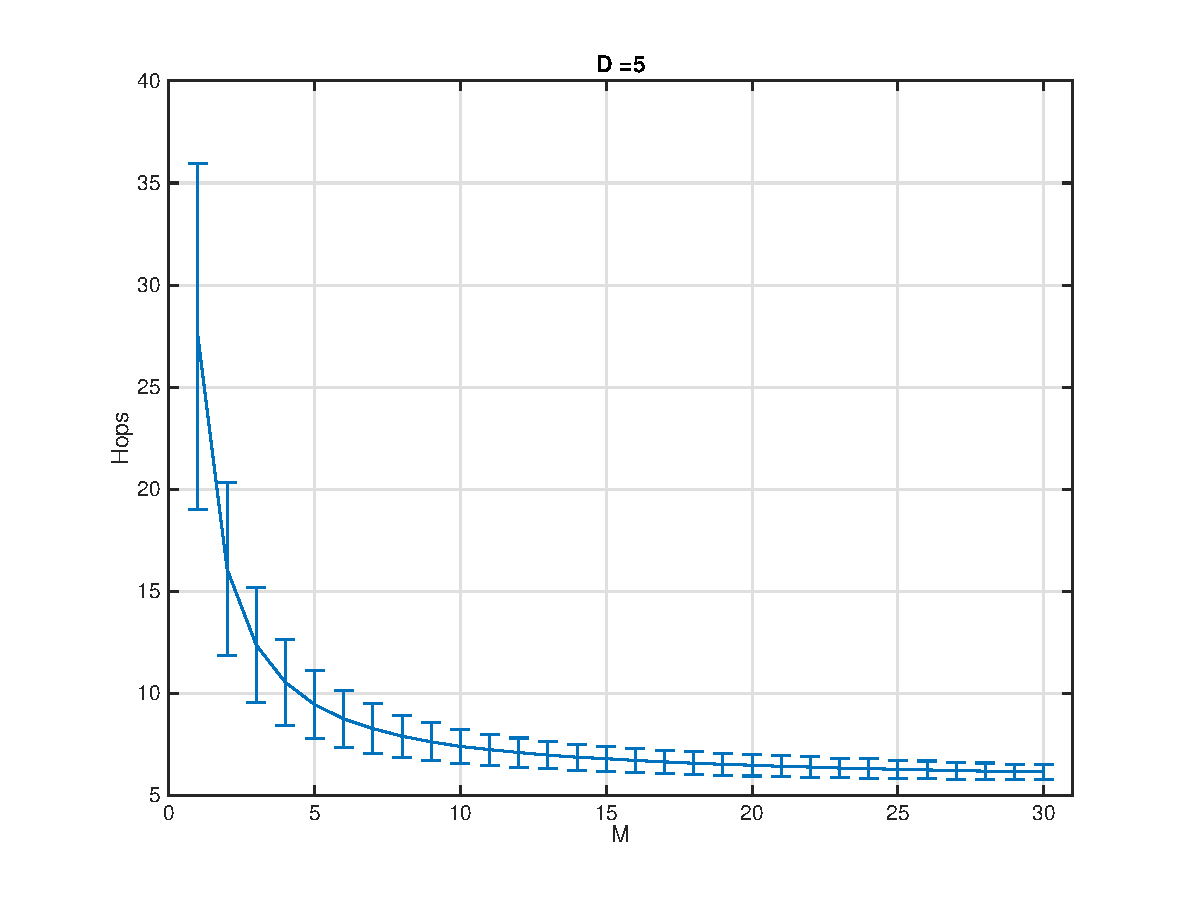
\includegraphics[width = 0.45\textwidth]{GeRaF_1}}
  \subfigure[$D = 10$]{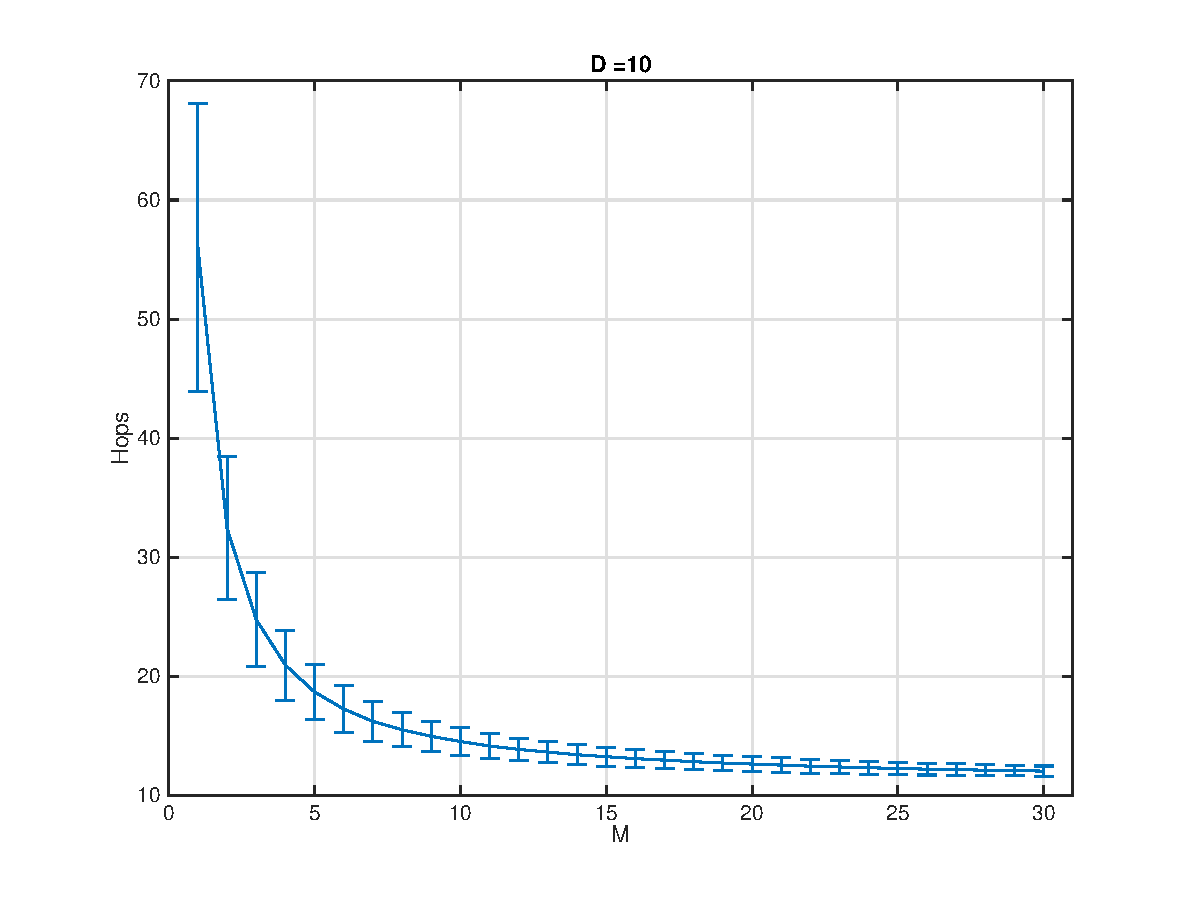
\includegraphics[width = 0.45\textwidth]{GeRaF_2}}
  \subfigure[$D = 20$]{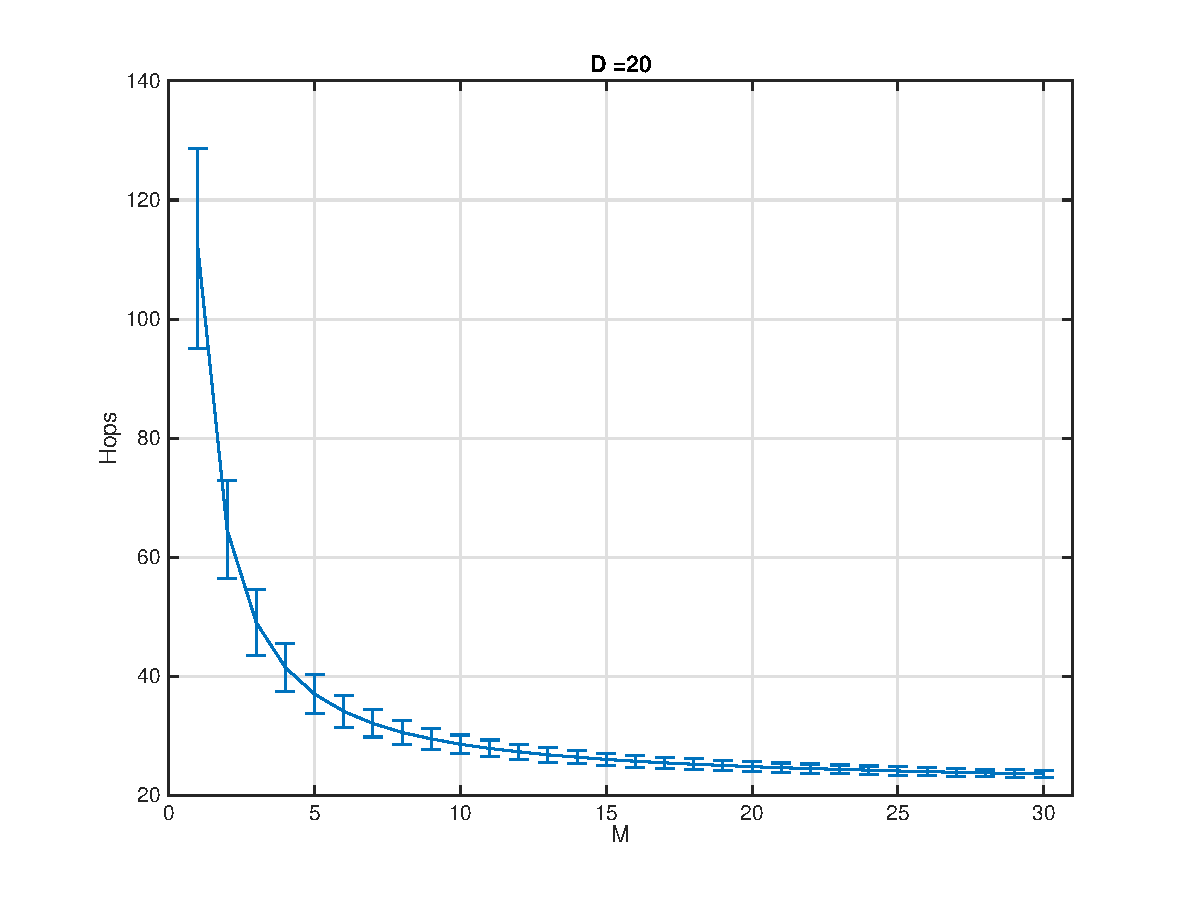
\includegraphics[width = 0.45\textwidth]{GeRaF_3}}
  \caption{Results for Montecarlo simulation for GeRaF}
  \label{fig:geraf1}
\end{figure}

An analytical bound can be computed too with a recursive computation. The distance $D$ from the source to the destination is quantized into small intervals. In particular let $\nu$ be the number of intervals of this kind inside the coverage radius. 

Let's consider as first an upper bound to the number of hops by assuming that if the relaying node is inside the $i$-th interval then it is placed at the beginning of this interval. Note that in this way the longest distance that can be covered in one hop is $(\nu - 1) / (\nu)$. With this approximation the intervals can be seen as states of a Markov chain. For $i = 0, \dots, \nu (D - 1) - 2$ (i.e. the intervals that are farther than 1 from the destination) the probability of going from the beginning of interval $i$ to the beginning of interval $k = i + j$ is 
\begin{equation}
\begin{cases}
  P(i, i + j) = e^{-M/pi A(j+1)} - e^{-M/pi A(j)}, \; j = 1, \nu-1 \\
  P(i, i) = e^{-M/pi A(1)} \; j = 0
\end{cases}
\end{equation}
where $A(j)$ is the area of the portion of the intersection between the coverage area circle and a circle at distance $D$, of radius $r = D - j/nu$. This area is given by
\begin{equation}
  A(j) = A(r, D) = 2\int_{D-1}^r a \cos^-1 \left( \frac{a^2 + D^2 - 1}{2aD} \right) da
\end{equation}
which is evaluated with Gauss-Legendre numerical integration. Indeed the primitive provided in \cite{tmc} generates a lower and upper bound which are above the upper bound of confidence interval the results of the Montecarlo simulation. 

The probability matrix $\mathbf{P}$ is computed with a MATLAB script and the last states (with index $D\nu - \nu - 1, \dots, D\nu -1 $) are considered absorbing states since they are in reach of the destination, thus
\begin{equation}
  P(i, i) = 1, \; i = D\nu - \nu - 1, \dots, D\nu -1 
\end{equation} 
Then the number of hops until absorption is 
\begin{equation}
\begin{cases}
  v(i) = 1, \; i = D\nu - \nu - 1, \dots, D\nu -1  \\
  v(i) = \frac{1+\sum_{j = 0}^{\nu - 1} P(i, i + j) v(i + j)}{1-P(i, i)}, \; i = 0, \dots, D\nu - \nu - 2
\end{cases}
\end{equation}

A lower bound can be computed too by assuming that each time the relay is inside the $i$-th interval then it is placed at the end of this interval. Therefore the distance covered by a single hop can range from 0 to 1. This is the second way of modeling the system as a Markov Chain, whose transition probability matrix is
\begin{equation}
\begin{cases}
  P(i, i + j) = e^{-M/pi A(j+1)} - e^{-M/pi A(j)}, & i = 0, \dots, \nu (D - 1) - 1, j = 1, \nu-1 \\
  P(i, i) = e^{-M/pi A(1)} & i = 0, \dots, \nu (D - 1) - 1, j = 0 \\
  P(i, i) = 1 & i = D\nu - \nu, \dots, D\nu 
\end{cases}
\end{equation}
and the number of hops until absorption is
\begin{equation}
\begin{cases}
  v(i) = 1, & i = D\nu - \nu , \dots, D\nu  \\
  v(i) = \frac{1+\sum_{j = 0}^{\nu} P(i, i + j) v(i + j)}{1-P(i, i)}, & i = 0, \dots, D\nu - \nu - 1
\end{cases}
\end{equation}

The results are in Figure~\ref{fig:geraf2}, note that for $\nu = 100$ the bounds are very close to each other and to the Montecarlo simulation (see~\ref{fig:geraf3} for a detail).

\begin{figure}[h!]
  \centering
  \subfigure[$D = 5$]{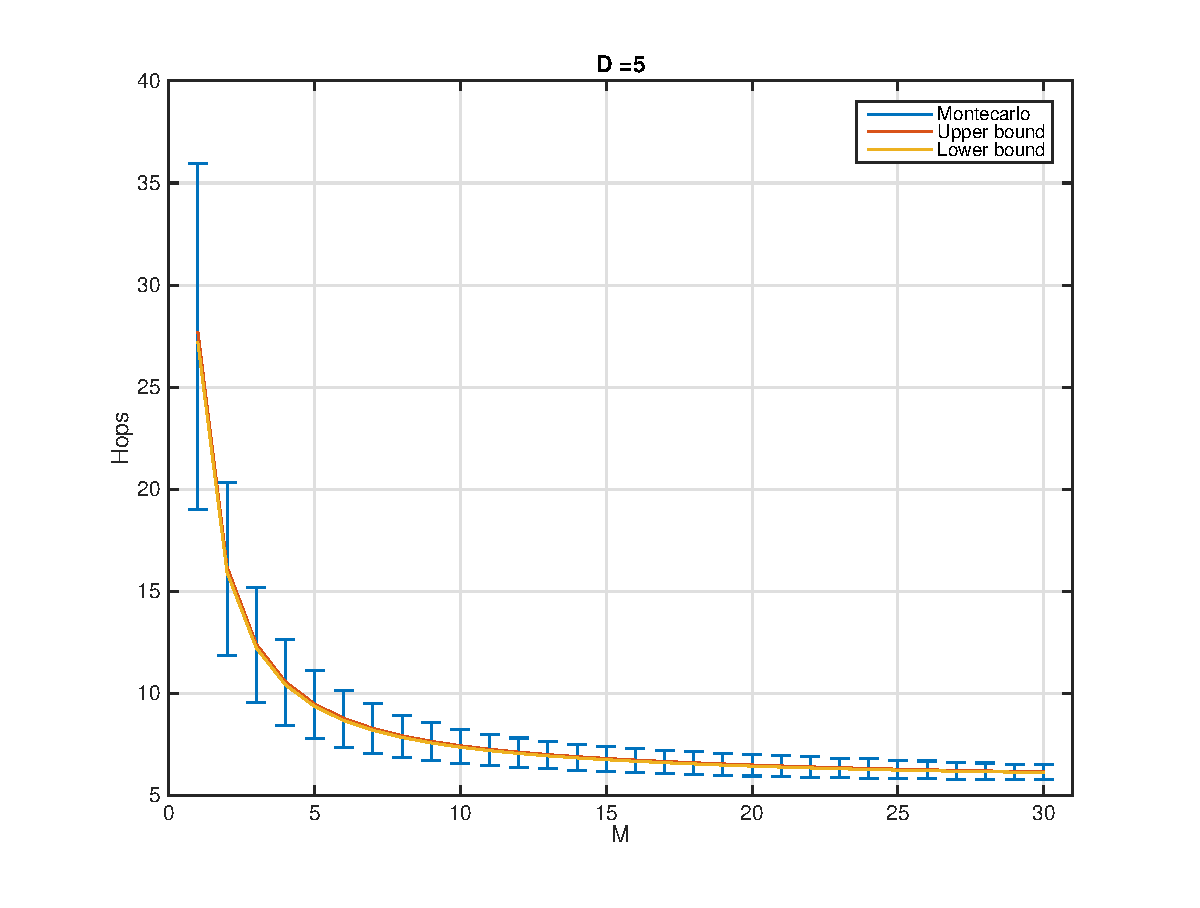
\includegraphics[width = 0.45\textwidth]{GeRaF_8}}
  \subfigure[$D = 10$]{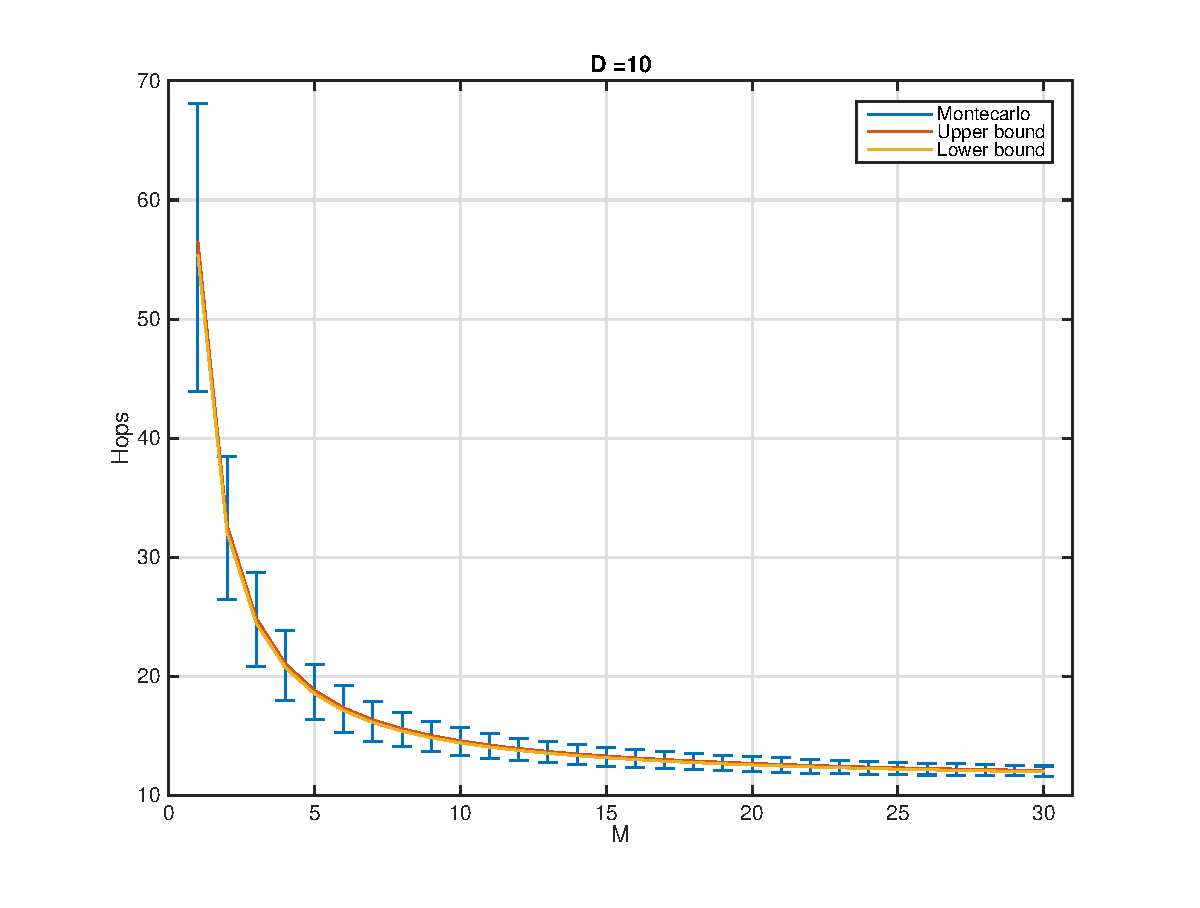
\includegraphics[width = 0.45\textwidth]{GeRaF_9}}
  \subfigure[$D = 20$]{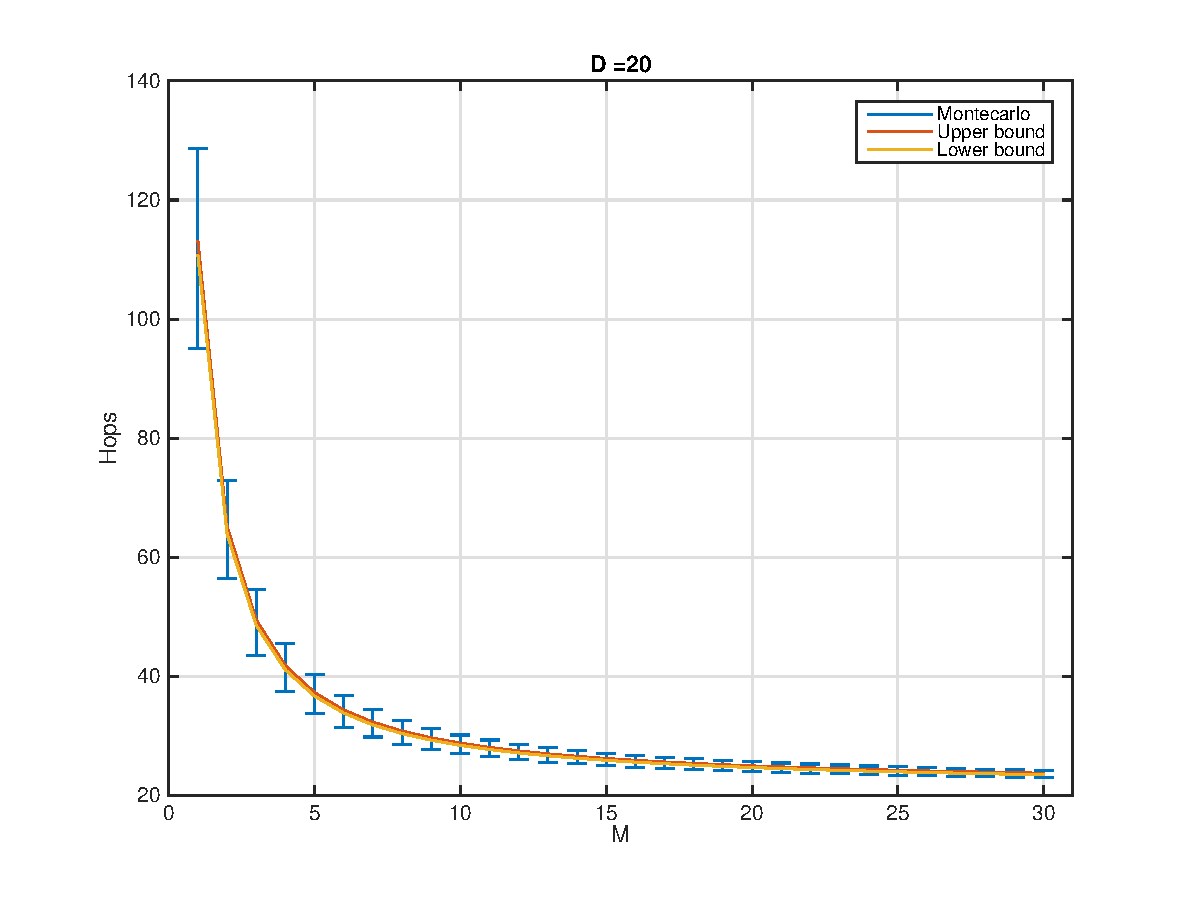
\includegraphics[width = 0.45\textwidth]{GeRaF_10}}
  \caption{Results for Montecarlo simulation and analytical bounds for GeRaF}
  \label{fig:geraf2}
\end{figure}

\begin{figure}[H]
  \centering
  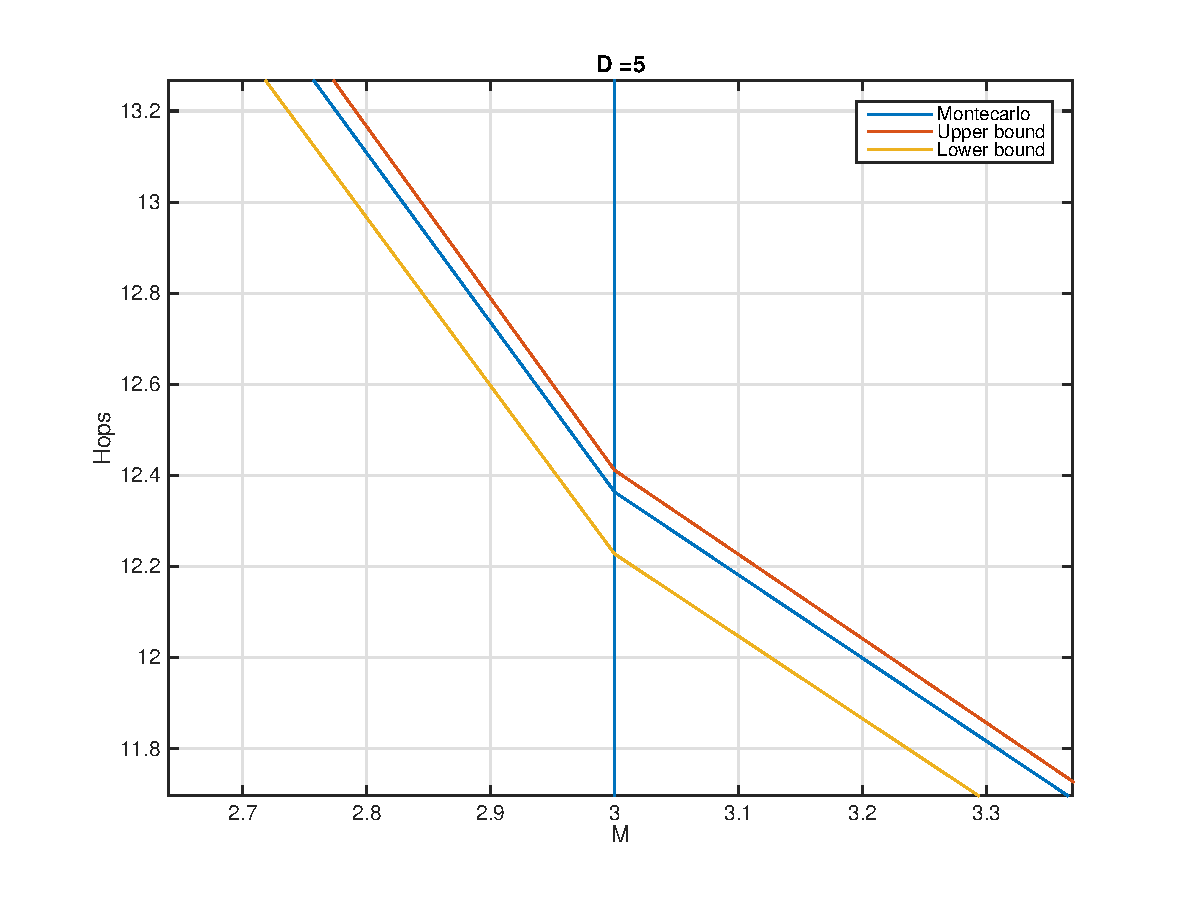
\includegraphics[width= 0.4\textwidth]{GeRaF_detail}
  \caption{Detail of the 3 curves for GeRaF Montecarlo and bounds, $D = 5$}
  \label{fig:geraf3}
\end{figure}

\FloatBarrier

\begin{thebibliography}{10}

\bibitem{leb}
Y. Le Boudec, Performance Evaluation of Computer and Communications Systems, EPFL, 2015

\bibitem{capture}
M. Zorzi and R. R. Rao, Capture and retransmission control in
mobile radio, IEEE J. Sel. Areas Commun., vol. SAC-12, no. 8, pp.
1289 - 1298, Oct. 1994

\bibitem{tmc}
Zorzi, M.; Rao, R.R., Geographic random forwarding (GeRaF) for ad hoc and sensor networks: multihop performance, Mobile Computing, IEEE Transactions on , vol.2, no.4, pp.337,348, Oct.-Dec. 2003


\end{thebibliography}

\end{document}
